\begin{enumerate}[label=\thesection.\arabic*.,ref=\thesection.\theenumi]
\numberwithin{equation}{enumi}
\item A position control system is shown in the figure below. The proportional controller used presently ($k_a$) is not providing satisfactory performance, Design appropriate controller to achieve maximum overshoot less than 15\%. Further, the load should be positioned with 1\% accuracy. For the motor to be used, load ad torque-speed curve is shown in figure below. System parameters are $J_m$ = 2 kg-$m^2$, $J_l$ = 10 kg-$m^2$, $f_m$ = 2 N-m-s/rad , k = 12 N-m/rad, sensitivity of error detector is $1/\pi$

\begin{figure}[!ht]
\centering
    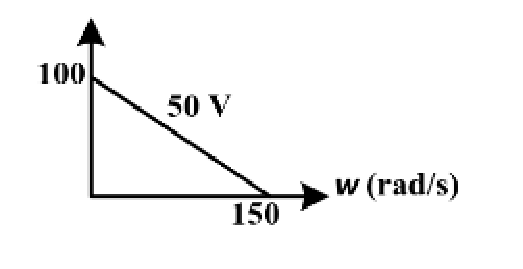
\includegraphics[width=150 pt,height = 75 pt]{./figs/ee18btech11019_1.eps}
  \caption{}
  \label{fig:ee18btech11019_fig1}
\end{figure}


\begin{figure}[!ht]
    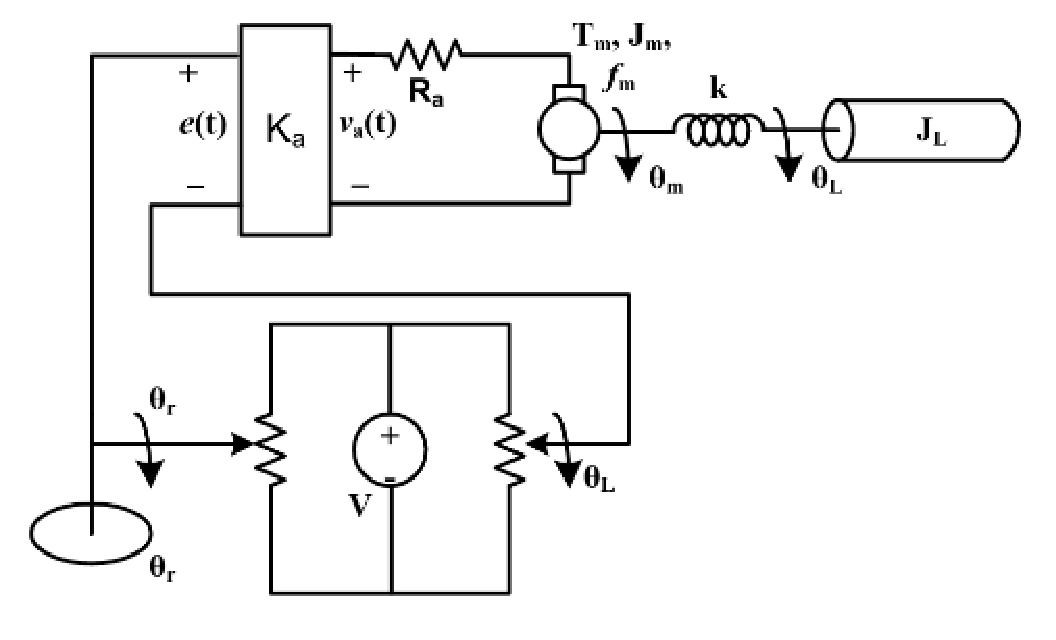
\includegraphics[width=\columnwidth]{./figs/ee18btech11019_2.eps}
  \caption{}
  \label{fig:ee18btech11019_fig2}
\end{figure}


\solution The following paragraph tells us about the components in the given position control system.\newline
We have, \newline
\textbf{Input}, it gives constant input = $\theta_r$\newline
\textbf{Plant}, Our original system\newline
\textbf{Potentiometer}, It convert position input and output to voltage.\newline
\textbf{Controller}, to get desired output.\newline

Below is the figure showing them,\newline
\begin{figure}[!ht]
    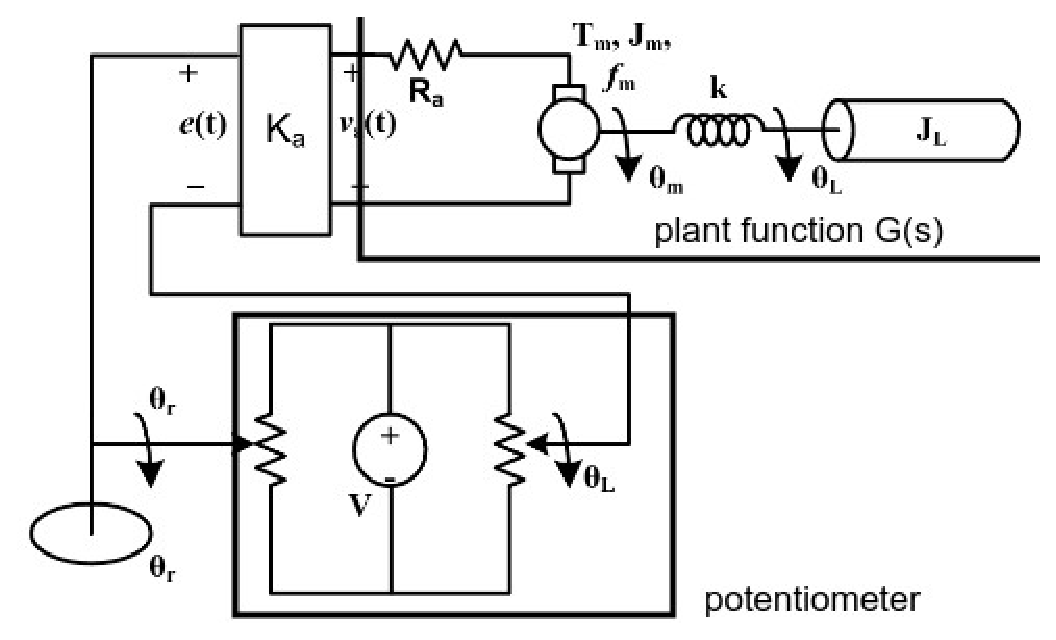
\includegraphics[width=\columnwidth]{./figs/ee18btech11019_3.eps}
  \caption{}
  \label{fig:ee18btech11019_fig3}
\end{figure}
Below is the block diagram, for the equivalent position control system.\newline
\begin{figure}[!ht]
    \begin{center}
		
		\resizebox{\columnwidth}{!}{\tikzset{
        block/.style = {draw, rectangle,
            minimum height=1cm,
            minimum width=2cm},
        input/.style = {coordinate,node distance=1cm},
        output/.style = {coordinate,node distance=4cm},
        arrow/.style={draw, -latex,node distance=2cm},
        pinstyle/.style = {pin edge={latex-, black,node distance=2cm}},
        sum/.style = {draw, circle, node distance=1cm},
}

\begin{tikzpicture}[node distance=2.5cm,auto,>=latex']
  \node [input, name=input] {};
  \node [sum, right of=input] (sum) {};
  \node [block, right of = sum] (block1) {$\frac{1}{\pi}$};
  \node [block, right of = block1] (block2) {Controller};
  \node [block, right of = block2] (block3) {Plant, G(s)};
  \node [output, right of= block3] (output) {};
  \draw [->] (input) -- node {i/p} (sum);
  \draw [->] (sum) -- node {e(t)} (block1);
  \draw [->] (block1) -- node {} (block2);
  \draw [->] (block2) -- node {} (block3);
  \draw [->] (block3) -- node [name =y] {o/p} (output);
  \draw [->] (y) -- ++ (0,-2) -| node [pos=0.99] {$-$} (sum);
\end{tikzpicture}}
	\end{center}
\caption{Block Circuit diagram}
\label{fig:circuit_diagram}
\end{figure}
Clearly from the question its negative feedback system and given sensitivity of system, it basically gets multiplied after error ( e(t) ), thus giving us a block of gain $\frac{1}{\pi}$\newline

\textbf{Calculating plant transfer function G(s)}:\newline\newline
\begin{table}[!ht]
\centering
%%%%%%%%%%%%%%%%%%%%%%%%%%%%%%%%%%%%%%%%%%%%%%%%%%%%%%%%%%%%%%%%%%%%%%
%%                                                                  %%
%%  This is the header of a LaTeX2e file exported from Gnumeric.    %%
%%                                                                  %%
%%  This file can be compiled as it stands or included in another   %%
%%  LaTeX document. The table is based on the longtable package so  %%
%%  the longtable options (headers, footers...) can be set in the   %%
%%  preamble section below (see PRAMBLE).                           %%
%%                                                                  %%
%%  To include the file in another, the following two lines must be %%
%%  in the including file:                                          %%
%%        \def\inputGnumericTable{}                                 %%
%%  at the beginning of the file and:                               %%
%%        \input{name-of-this-file.tex}                             %%
%%  where the table is to be placed. Note also that the including   %%
%%  file must use the following packages for the table to be        %%
%%  rendered correctly:                                             %%
%%    \usepackage[latin1]{inputenc}                                 %%
%%    \usepackage{color}                                            %%
%%    \usepackage{array}                                            %%
%%    \usepackage{longtable}                                        %%
%%    \usepackage{calc}                                             %%
%%    \usepackage{multirow}                                         %%
%%    \usepackage{hhline}                                           %%
%%    \usepackage{ifthen}                                           %%
%%  optionally (for landscape tables embedded in another document): %%
%%    \usepackage{lscape}                                           %%
%%                                                                  %%
%%%%%%%%%%%%%%%%%%%%%%%%%%%%%%%%%%%%%%%%%%%%%%%%%%%%%%%%%%%%%%%%%%%%%%



%%  This section checks if we are begin input into another file or  %%
%%  the file will be compiled alone. First use a macro taken from   %%
%%  the TeXbook ex 7.7 (suggestion of Han-Wen Nienhuys).            %%
\def\ifundefined#1{\expandafter\ifx\csname#1\endcsname\relax}


%%  Check for the \def token for inputed files. If it is not        %%
%%  defined, the file will be processed as a standalone and the     %%
%%  preamble will be used.                                          %%
\ifundefined{inputGnumericTable}

%%  We must be able to close or not the document at the end.        %%
	\def\gnumericTableEnd{\end{document}}


%%%%%%%%%%%%%%%%%%%%%%%%%%%%%%%%%%%%%%%%%%%%%%%%%%%%%%%%%%%%%%%%%%%%%%
%%                                                                  %%
%%  This is the PREAMBLE. Change these values to get the right      %%
%%  paper size and other niceties.                                  %%
%%                                                                  %%
%%%%%%%%%%%%%%%%%%%%%%%%%%%%%%%%%%%%%%%%%%%%%%%%%%%%%%%%%%%%%%%%%%%%%%

	\documentclass[12pt%
			  %,landscape%
                    ]{report}
       \usepackage[latin1]{inputenc}
       \usepackage{fullpage}
       \usepackage{color}
       \usepackage{array}
       \usepackage{longtable}
       \usepackage{calc}
       \usepackage{multirow}
       \usepackage{hhline}
       \usepackage{ifthen}




%%  End of the preamble for the standalone. The next section is for %%
%%  documents which are included into other LaTeX2e files.          %%
\else

%%  We are not a stand alone document. For a regular table, we will %%
%%  have no preamble and only define the closing to mean nothing.   %%
    \def\gnumericTableEnd{}

%%  If we want landscape mode in an embedded document, comment out  %%
%%  the line above and uncomment the two below. The table will      %%
%%  begin on a new page and run in landscape mode.                  %%
%       \def\gnumericTableEnd{\end{landscape}}
%       \begin{landscape}


%%  End of the else clause for this file being \input.              %%
\fi

%%%%%%%%%%%%%%%%%%%%%%%%%%%%%%%%%%%%%%%%%%%%%%%%%%%%%%%%%%%%%%%%%%%%%%
%%                                                                  %%
%%  The rest is the gnumeric table, except for the closing          %%
%%  statement. Changes below will alter the table's appearance.     %%
%%                                                                  %%
%%%%%%%%%%%%%%%%%%%%%%%%%%%%%%%%%%%%%%%%%%%%%%%%%%%%%%%%%%%%%%%%%%%%%%

\providecommand{\gnumericmathit}[1]{#1} 
%%  Uncomment the next line if you would like your numbers to be in %%
%%  italics if they are italizised in the gnumeric table.           %%
%\renewcommand{\gnumericmathit}[1]{\mathit{#1}}
\providecommand{\gnumericPB}[1]%
{\let\gnumericTemp=\\#1\let\\=\gnumericTemp\hspace{0pt}}
 \ifundefined{gnumericTableWidthDefined}
        \newlength{\gnumericTableWidth}
        \newlength{\gnumericTableWidthComplete}
        \newlength{\gnumericMultiRowLength}
        \global\def\gnumericTableWidthDefined{}
 \fi
%% The following setting protects this code from babel shorthands.  %%
 \ifthenelse{\isundefined{\languageshorthands}}{}{\languageshorthands{english}}
%%  The default table format retains the relative column widths of  %%
%%  gnumeric. They can easily be changed to c, r or l. In that case %%
%%  you may want to comment out the next line and uncomment the one %%
%%  thereafter                                                      %%
\providecommand\gnumbox{\makebox[0pt]}
%%\providecommand\gnumbox[1][]{\makebox}

%% to adjust positions in multirow situations                       %%
\setlength{\bigstrutjot}{\jot}
\setlength{\extrarowheight}{\doublerulesep}

%%  The \setlongtables command keeps column widths the same across  %%
%%  pages. Simply comment out next line for varying column widths.  %%
\setlongtables

\setlength\gnumericTableWidth{%
	80pt+%
	50pt+%
	60pt+%
0pt}
\def\gumericNumCols{3}
\setlength\gnumericTableWidthComplete{\gnumericTableWidth+%
         \tabcolsep*\gumericNumCols*2+\arrayrulewidth*\gumericNumCols}
\ifthenelse{\lengthtest{\gnumericTableWidthComplete > \linewidth}}%
         {\def\gnumericScale{\ratio{\linewidth-%
                        \tabcolsep*\gumericNumCols*2-%
                        \arrayrulewidth*\gumericNumCols}%
{\gnumericTableWidth}}}%
{\def\gnumericScale{1}}

%%%%%%%%%%%%%%%%%%%%%%%%%%%%%%%%%%%%%%%%%%%%%%%%%%%%%%%%%%%%%%%%%%%%%%
%%                                                                  %%
%% The following are the widths of the various columns. We are      %%
%% defining them here because then they are easier to change.       %%
%% Depending on the cell formats we may use them more than once.    %%
%%                                                                  %%
%%%%%%%%%%%%%%%%%%%%%%%%%%%%%%%%%%%%%%%%%%%%%%%%%%%%%%%%%%%%%%%%%%%%%%

\ifthenelse{\isundefined{\gnumericColA}}{\newlength{\gnumericColA}}{}\settowidth{\gnumericColA}{\begin{tabular}{@{}p{30pt*\gnumericScale}@{}}x\end{tabular}}
\ifthenelse{\isundefined{\gnumericColC}}{\newlength{\gnumericColC}}{}\settowidth{\gnumericColC}{\begin{tabular}{@{}p{160pt*\gnumericScale}@{}}x\end{tabular}}
\begin{tabular}[c]{%
	b{\gnumericColA}%	
	b{\gnumericColC}%
	}

%%%%%%%%%%%%%%%%%%%%%%%%%%%%%%%%%%%%%%%%%%%%%%%%%%%%%%%%%%%%%%%%%%%%%%
%%  The longtable options. (Caption, headers... see Goosens, p.124) %%
%	\caption{The Table Caption.}             \\	%
% \hline	% Across the top of the table.
%%  The rest of these options are table rows which are placed on    %%
%%  the first, last or every page. Use \multicolumn if you want.    %%

%%  Header for the first page.                                      %%
%	\multicolumn{3}{c}{The First Header} \\ \hline 
%	\multicolumn{1}{c}{colTag}	%Column 1
%	&\multicolumn{1}{c}{colTag}	%Column 2
%	&\multicolumn{1}{c}{colTag}	\\ \hline %Last column
%	\endfirsthead

%%  The running header definition.                                  %%
%	\hline
%	\multicolumn{3}{l}{\ldots\small\slshape continued} \\ \hline
%	\multicolumn{1}{c}{colTag}	%Column 1
%	&\multicolumn{1}{c}{colTag}	%Column 2
%	&\multicolumn{1}{c}{colTag}	\\ \hline %Last column
%	\endhead

%%  The running footer definition.                                  %%
%	\hline
%	\multicolumn{3}{r}{\small\slshape continued\ldots} \\
%	\endfoot

%%  The ending footer definition.                                   %%
%	\multicolumn{3}{c}{That's all folks} \\ \hline 
%	\endlastfoot
%%%%%%%%%%%%%%%%%%%%%%%%%%%%%%%%%%%%%%%%%%%%%%%%%%%%%%%%%%%%%%%%%%%%%%


	
\hhline{|-|-}
	 \multicolumn{1}{|p{\gnumericColA}|}%
	{\gnumericPB{\centering}\textbf{Parameter}}
	&\multicolumn{1}{p{\gnumericColC}|}%
	{\gnumericPB{\centering}\textbf{Description}}

\\

	

\hhline{|--|}
	 \multicolumn{1}{|p{\gnumericColA}|}%
	{\gnumericPB{\centering}$\Vec{T_{m}}$}
	&\multicolumn{1}{p{\gnumericColC}|}%
	{\gnumericPB{\centering}Torque applied on motor due to armature voltage}
	
	
\\

	
	\hhline{|--|}
	 \multicolumn{1}{|p{\gnumericColA}|}%
	{\gnumericPB{\centering}$R_a$}
	&\multicolumn{1}{p{\gnumericColC}|}%
	{\gnumericPB{\centering}Motor parameter}
\\

	
	\hhline{|--|}
	 \multicolumn{1}{|p{\gnumericColA}|}%
	{\gnumericPB{\centering}$K_t$}
	&\multicolumn{1}{p{\gnumericColC}|}%
	{\gnumericPB{\centering}Motor parameter}
\\

	
	\hhline{|--|}
	 \multicolumn{1}{|p{\gnumericColA}|}%
	{\gnumericPB{\centering}$K_b$}
	&\multicolumn{1}{p{\gnumericColC}|}%
	{\gnumericPB{\centering}Motor parameter}

\\
	\hhline{|--|}
	 \multicolumn{1}{|p{\gnumericColA}|}%
	{\gnumericPB{\centering}$V_{a}$}
	&\multicolumn{1}{p{\gnumericColC}|}%
	{\gnumericPB{\centering}Armature voltage of DC Motor}

\\
	
	\hhline{|--|}
	 \multicolumn{1}{|p{\gnumericColA}|}%
	{\gnumericPB{\centering}$J_m$}
	&\multicolumn{1}{p{\gnumericColC}|}%
	{\gnumericPB{\centering}Moment of inertia of motor}

\\

	\hhline{|--|}
	 \multicolumn{1}{|p{\gnumericColA}|}%
	{\gnumericPB{\centering}$J_L$}
	&\multicolumn{1}{p{\gnumericColC}|}%
	{\gnumericPB{\centering}Moment of inertia of load}

\\

	\hhline{|--|}
	 \multicolumn{1}{|p{\gnumericColA}|}%
	{\gnumericPB{\centering}$\bm{\theta_{m}}$}
	&\multicolumn{1}{p{\gnumericColC}|}%
	{\gnumericPB{\centering}Angular position of motor}

\\

	
	\hhline{|--|}
	 \multicolumn{1}{|p{\gnumericColA}|}%
	{\gnumericPB{\centering}$\bm{\theta_{L}}$}
	&\multicolumn{1}{p{\gnumericColC}|}%
	{\gnumericPB{\centering} Angular position of Load}

\\
	\hhline{|--|}
	 \multicolumn{1}{|p{\gnumericColA}|}%
	{\gnumericPB{\centering}$f_{m}$}
	&\multicolumn{1}{p{\gnumericColC}|}%
	{\gnumericPB{\centering}Viscous friction on motor}

\\
	\hhline{|--|}
	 \multicolumn{1}{|p{\gnumericColA}|}%
	{\gnumericPB{\centering} k }
	&\multicolumn{1}{p{\gnumericColC}|}%
	{\gnumericPB{\centering}Angular spring constant}

\\

\hhline{|-|-}
\end{tabular}

\ifthenelse{\isundefined{\languageshorthands}}{}{\languageshorthands{\languagename}}
\gnumericTableEnd
\caption{parameters description}
\label{table:ee18btech110019_2}
\end{table}
$V_a(t)$ is the input to the plant and output is $\theta_L$\newline
We know that,\newline
The relation between armature voltage and torque $T_m$ \newline
directly taking result from book control systems engineering by norman-nise, $6^{th}$ edition. Equation no. 2.156 (on page number 82)\newline
\begin{align}
    T_m(s)\frac{R_a}{K_t} + K_bs\theta_m(s)  &=  V_a(s)
\end{align}
Considering free-body diagram of motor we get,\newline 
$T_m$ is counter balanced by \newline 1) inertial forces(due to $J_m$)\newline 2) viscous frictional force($f_m$) \newline 3) the spring force($k\theta_m$),\newline but also the counter spring force is exerted on motor(in the same direction as $T_m$) due to presence of finite load ($k\theta_L$)\newline
Below is the equation:\newline
\begin{align}
    (J_ms^2 + f_ms + k)\theta_m(s) - k\theta_L(s)  &=  T_m(s) 
\end{align}
Now, considering free body diagram on  the load, we get\newline
$K\theta_m$ is the driving force\newline
Inertial force($J_l$) and opposing spring force ($K\theta_L$) are the opposing forces.\newline
Below is the equation:\newline
\begin{align}
   (J_Ls^2 + k)\theta_L(s)  &=  k\theta_m(s)
\end{align}
Where, \newline
From the graph given in question:\newline
V is 50 V\newline
$T_{stall}$ is torque when $\omega$ =0, i.e. = 100\newline
$\omega_{no-load}$ is $\omega$ when T is 0, i.e. = 150\newline
\begin{align}
    \frac{R_a}{K_t} &= \frac{V}{T_{stall}} = \frac{50}{100} = \frac{1}{2}\\
    k_b &= \frac{V}{w_{no-load}} = \frac{50}{150} = \frac{1}{3}
\end{align}
On Solving we get,\newline
\begin{align}
G(s) &= \frac{\theta_L(s)}{V_a(s)}\\
G(s) &= \frac{1}{\frac{5}{6}s^4 + \frac{10}{9}s^3 + 6S^2 + \frac{4}{3}s}
\end{align}


Now, lets design a controller for the following plant function to get desired output.\newline
1) Steady state error is 1\% \newline
2) Peak overshoot is less than 15\% \newline

\textbf{Steady state error condition}:\newline
Considering the closed-loop gain of plant function.\newline
Steady state error is given by,\newline
\begin{align}
    &= \frac{G(s)}{1 + G(s)}
\end{align}
We know that, steady state output is given by 
\begin{align}
    \lim_{s\to0} sR(s)\myvec{\frac{G(s)}{1 + G(s)}}\\
    R(s) = \frac{1}{s}\\
   \text{ steady state output} &= 1
\end{align}
Given we have 1\% error,\newline
Steady state error is given by,\newline
\begin{align}
    e_{ss} &= \lim_{s\to0} \myvec{\frac{sR(s)}{1 + G(s)}}
\end{align}   
Here, as we see we get 0 steady state error, therefore to make it finite we cascade a differentiator to the plant function\newline
Below is the block representation\newline
\begin{figure}[!ht]
    \begin{center}
			\resizebox{\columnwidth}{!}{
\begin{circuitikz}[scale =2]

	\draw
	% Drawing a npn transistor
	(0,0) node[npn](npn1){} 
	% Making connections from transistor using relative coordinates
	% Labelling the transistor
	(npn1.B) to[C=$C_1$](-1,0) --(-1,-3)--++(3,0)
	%(npn1.C) --++(0,0.5) --++(0.75,0) to[R=R](0.75,-1.25) -- (0,-1.25)
	(0.75,-1.25) -- (0,-1.25)
	(npn1.E) to[R= $R_4$](0,-1) to node[ground]{}(0,-1.25);
	\draw (0.75,1.25) --++(1.25,0) to[L=$L_1$](2,-1.25)--(0.75,-1.25)
	(2,-1.25) to[L=$L_2$](2,-3) -- (1,-3)
	(2,1.25) -- (3,1.25) to[C=C](3,-3)--(2,-3)
	(npn1.B) to[R=$R_2$](-0.4,1.25)
	(npn1.B) to[R = $R_3$](-0.4,-1.25) -- (0, -1.25)
	(npn1.C) --(0.5,0.4) to[C = $C_1$](0.5,1.25)
	(npn1.C) to[R=$R_1$](0,1.25)
	(-0.4,1.25) -- (0,1.25)
	(0.5,1.25) -- (0.75,1.25)
	(-0.4,1.25) -- (-0.5,1.25)node[left]{12 V }
	;
	
\end{circuitikz}
}
	\end{center}
\caption{Cascading a differentiator}
\label{fig:block2}
\end{figure}\newline
As, $\frac{1}{\pi}$ is cascade to our plant, so directly multiplying for sake of simplicity.
\begin{align}
    \lim_{s\to0} \myvec{\frac{sR(s)}{1 + G^{'}(s)}} &= 0.01\\
    \lim_{s\to0} \frac{1}{1 + \frac{1}{\pi}(Ks)G(s)} &= 0.01
\end{align} 
Solving, \\
\begin{align}
    K &= 132\pi
\end{align}
Therefor, the overall system as can be written as,\newline
\begin{align}
    G(s) &= \frac{132}{\frac{5}{6}s^3 + \frac{10}{9}s^2 + 6s + \frac{4}{3}}
\end{align}
\textbf{Peak overshoot:}\\
Lets use a PID-controller for this purpose, 
So, as we want peak overshoot to be less than 15\%.\newline
So, this is the final block diagram\newline\newline
\begin{figure}[!ht]
    \begin{center}
			\resizebox{\columnwidth}{!}{\tikzset{
        block/.style = {draw, rectangle,
            minimum height=1cm,
            minimum width=2cm},
        input/.style = {coordinate,node distance=1cm},
        output/.style = {coordinate,node distance=4cm},
        arrow/.style={draw, -latex,node distance=2cm},
        pinstyle/.style = {pin edge={latex-, black,node distance=2cm}},
        sum/.style = {draw, circle, node distance=1cm},
}

\begin{tikzpicture}[node distance=2.5cm,auto,>=latex']
  \node [input, name=input] {};
  \node [sum, right of=input] (sum) {};
  \node [block, right of = sum] (block1) {Controller};
  \node [block, right of = block1] (block2) {G(s)};
  \node [output, right of= block2] (output) {};
  \draw [->] (input) -- node {i/p} (sum);
  \draw [->] (sum) -- node {} (block1);
  \draw [->] (block1) -- node {} (block2);
  \draw [->] (block2) -- node [name =y] {o/p} (output);
  \draw [->] (y) -- ++ (0,-2) -| node [pos=0.99] {$-$} (sum);
\end{tikzpicture}}
	\end{center}
\caption{Block diagram so far}
\label{fig:block3}
\end{figure}

General expression for PID-controller given by:
\begin{align}
     K_{p}\brak{1 + T_{d}s + \frac{1}{T_{i}s}}
\end{align}
For it to satisfy our steady state condition, \newline we will take $K_P$ = 1.\newline
And also \textbf{cascading it with a differentiator of gain = $T_i$}, to remove the pole and thus maintaining or steady state value.\newline
Final transfer function is given by,\newline
\begin{align}
    &= \frac{132\brak{S + T_{d}s^2 + \frac{1}{T_{i}}}T_i}{\frac{5}{6}s^3 + \frac{10}{9}s^2 + 6s + \frac{4}{3}}
\end{align}
Considering $2^{nd}$ order approximation.\newline
Relation between \%OS = 15\% and Damping ratio
\begin{align}
\zeta &= \frac{-\ln(\%OS/100)}{\sqrt{(\pi)^2 + (\ln(\%OS/100))^2}}
\end{align}
\begin{align}
\implies\zeta &= 0.517 
\end{align}
Phase Margin for a Damping ratio is given by Eq \eqref{eq:ee18btech11030}  
\begin{align}
\label{eq:ee18btech11030}
\phi_{m} &= 90\degree - \arctan\brak{\frac{\sqrt{-2\zeta^2+\sqrt{1+4\zeta^4}}}{2\zeta}}
\end{align}
\begin{align}
\implies \phi_{m} &= 53.17\degree
\end{align}

Adding a correction factor, to compensate for the phase gain,  to our phase margin we get, 
\begin{align}
    \phi_{m} = 70\degree
\end{align}
Now, solving for the values,\newline
\begin{align}
    \abs{G(j\omega)} &= \frac{132 T_i\sqrt{\brak{1/T_i-T_d\omega ^{2}}^2 + \omega ^2}}{\sqrt{\brak{4/3-10\omega ^2/9}^2 + \brak{6 \omega ^2 -5\omega ^3/6}}}\\
    &= 1
\end{align}
And,\newline
\begin{align}
    \arctan\brak{\frac{\omega}{1/T_i-T_d\omega ^{2}}} - \arctan\brak{\frac{6 \omega ^2 -5\omega ^3/6}{4/3-10\omega ^2/9}}\\
    = 70\degree-180\degree = -110\degree       
\end{align}
Solving one the best fits we get is,\newline
\begin{align}
    T_i = \frac{100}{132}\\
    T_d = 0.1\brak{\frac{132}{100}}\\
    \omega = 17.07
\end{align}
\textbf{Final transfer function is given by}:
\begin{align}
 = \frac{13.2s^2+100s+132}{5/6s^3 + 10/9s^2 + 6s + 4/3}
\end{align}
\textbf{Below is the figure for the magnitude and phase plot of the function}\newline
Following's the code:
\begin{lstlisting}
codes/ee18btech11019_1.py
\end{lstlisting}

\begin{figure}[!ht]
    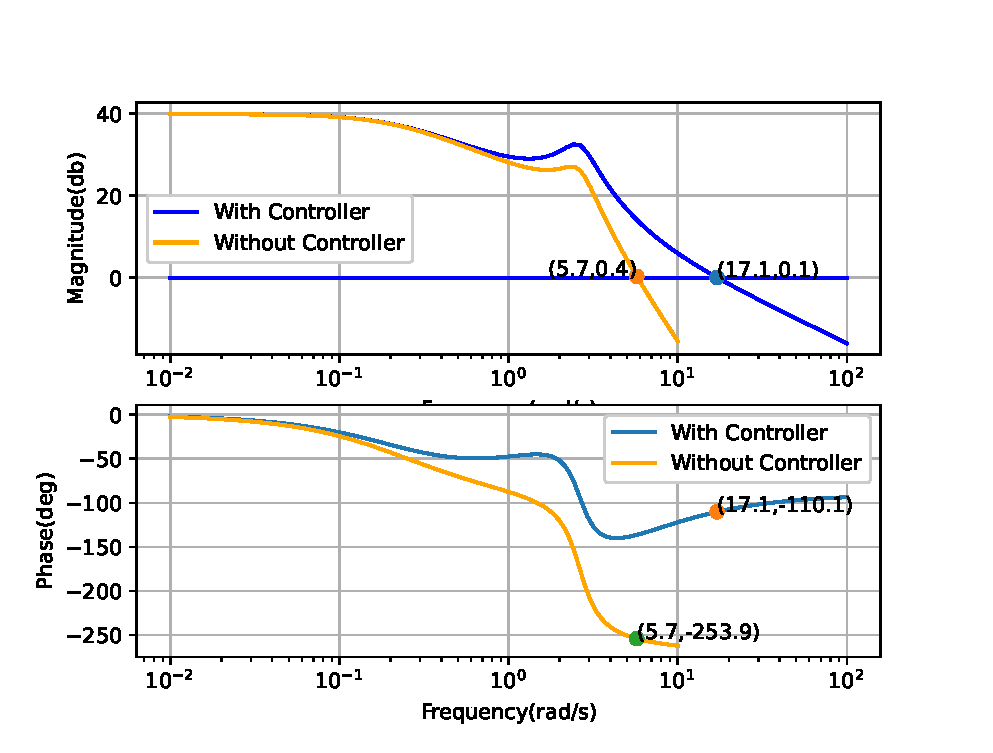
\includegraphics[width=\columnwidth]{./figs/ee18btech11019_6.eps}
  \caption{Mag and phase plot comparison}
  \label{fig:ee18btech11019_fig_plot}
\end{figure}
\textbf{Below is the figure for the output comparison in time domain for unit step input}:\newline
Following's the code:
\begin{lstlisting}
codes/ee18btech11019_2.py
\end{lstlisting}

\begin{figure}[!ht]
    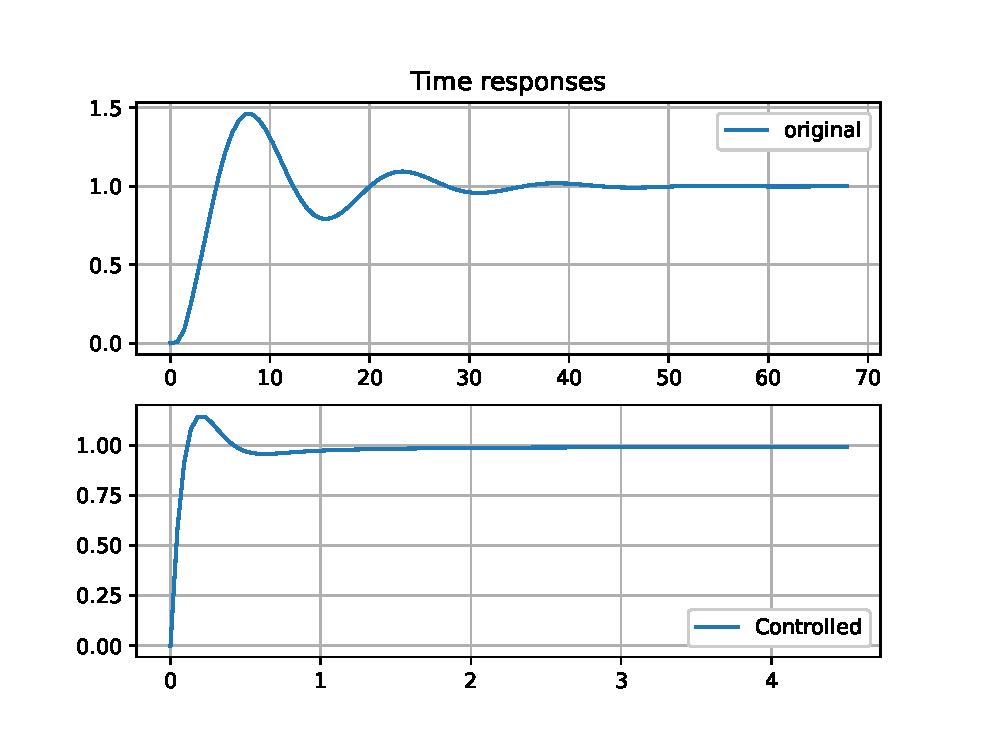
\includegraphics[width=\columnwidth]{./figs/ee18btech11019_7.eps}
  \caption{Time response}
  \label{fig:ee18btech11019_fig_val}
\end{figure}
\textbf{Here, is the table of expected value and obtained value}:\newline
Originally, we had around 50\% peak overshoot, without controller

\begin{table}[!ht]
\centering
\begin{enumerate}[label=\thesection.\arabic*.,ref=\thesection.\theenumi]
\numberwithin{equation}{enumi}

\item Fig. \label{fig:ee18btech11019_hart} shows a Hartley oscillator.

\begin{figure}[ht]
    \begin{center}
	    \resizebox{\columnwidth}{!}{\begin{circuitikz} [scale=2]  \draw 
(0,0) node[op amp] (opamp) [scale=2] {}
(opamp.-) -- (-3,0.5) to [R=$R_1$] (-5,0.5) -- (-6,0.5) -- (-6,-2) to [L=$L_2$] (-4,-2)
-- (-1,-2) to[L=$L_1$] (1,-2) -- (1,0) {};
\node[draw,box] (A) at (1.5,-0.7) {$V_{out}$};
\draw (-6,-2) -- (-6,-3)  to [C=$C$] (1,-3) -- (1,-2) 

(opamp.-) to[short,*-] ++(0,1) coordinate (leftC)
to[R=$R_2$] (leftC -| opamp.out)
to[short,-*] (opamp.out) to [short,-o] (1.5,0) to (1.5,-0.5) {}
(opamp.+) -- (-3,-0.5) to [R=$R_3$] (-5,-0.5) node[ground] [scale=2] {};
\draw (-2,-0.5) -- (-2,-2);


\end{circuitikz}
}
	\end{center}
\caption{Hartley oscillator}
\label{fig:ee18btech11019_hart}
\end{figure}
Draw the equivalent block diagram.
\solution  The block diagram is available in Fig. \label{fig:ee18btech11019_hart_block}
\begin{figure}[!ht]
    \begin{center}
		
		\resizebox{\columnwidth}{!}{\tikzset{
        amp/.style = {regular polygon, regular polygon sides=3,
              draw, fill=white, text width=1em,
              inner sep=1mm, outer sep=0mm,
              shape border rotate=-90},
        block/.style = {draw, rectangle,
            minimum height=1cm,
            minimum width=2cm},
        input/.style = {coordinate,node distance=1cm},
        output/.style = {coordinate,node distance=4cm},
        arrow/.style={draw, -latex,node distance=2cm},
        pinstyle/.style = {pin edge={latex-, black,node distance=2cm}},
        sum/.style = {draw, circle, node distance=1cm},
}

\begin{tikzpicture}[node distance=2.5cm,auto,>=latex']
  \node [input, name=input] {};
  \node [sum, right of=input] (sum) {};
  \node [amp, right of = sum] (block1) {$A$};
  \node [output, right of= block1] (output) {};
  \node [block, below of = block1] (block2) {$B$};
  \draw [->] (input) -- node {$V_{in}$} (sum);
  \draw [->] (sum) -- node {$V_{in} + BV_{out}$} (block1);
  \draw [->] (block1) -- node [name =y] {$V_{out}$} (output);
  \draw [->] (y) |- node [above,pos=0.79] {$V_{out}$} (block2) ;
  \draw [->] (block2) -| node  {$BV_{out}$} (sum) ;
\end{tikzpicture}
} %block diagram
	\end{center}
\caption{block diagram for oscillator}
\label{fig:ee18btech11019_hart_block}
\end{figure}
%
\item Find the gain of the oscillator. 
\\
\solution The control system in Fig. \ref{fig:ee18btech11019_hart_block} has positive feedback.  Hence, the gain is 

\begin{align}
    G = \frac{G(s)}{1-G(s)H(s)}
\label{eq:ee18btech11019_gain}
\end{align}
%
\item Find $G(s)$ and $H(s)$.
\\
\solution From figure \ref{fig:ee18btech11019_hart_block}
Oscillators gain can be given as follows:\\
\begin{align}
    A(V_{in} + BV_{out}) =V_{out}\\
    A(V_{in} = (1-AB)V_{out}\\
    \frac{V_{out}}{V_{in}} = \frac{A}{1 - AB}
\end{align}
%
resulting in \eqref{eq:ee18btech11019_gain}.\\



\item State the condition for sustained oscillations. Justify.

\solution Condition for sustained oscillation is given by\\
\begin{align}
    AB = 1
\end{align}
Along with, total phase gain o the circuit should be 0 or 2$\pi$\\
\textbf{Justification:} as, when $ AB =1 $, gain becomes infinity, and theoretically we can get output, without actually providing input\\
Total phase gain should be so, as we want our signal to be in phase after every loop traversal.\\


\item Find $A$ and $B$.

\solution Consider the below circuit fig \ref{fig:ee18btech11019_block2},its basic form of a LC oscillator.\\
%\begin{figure}[!ht]
%    \begin{center}
%		\resizebox{\columnwidth}{!}{\begin{circuitikz} 
(0,0) node[op amp] (opamp) [scale=2] {}
\draw
(0,0) -- (4,0) node[label = $V_{out}$]
  to [european resistor = $Z_2$]  (4,-4)   -- (0,-4)node[ground] {} to[european resistor = $Z_1$] (0,-2) 
  to[european resistor = $Z_3$] (0,0);
  \draw 
    (-2,0) node[op amp] (opamp) {} 
    (0,0) -- (opamp.out)
    (opamp.+)--(-4,-0.5)--(-4,-1)node[ground] {}
  (0,-2)--(-6,-2)--(-6,0.5) -- (opamp.-);
  

\end{circuitikz} 
}
%		
%	\end{center}
%\caption{block diagram for oscillator}
%\label{fig:ee18btech11019_block2}
%\end{figure}
The above figure \ref{fig:ee18btech11019_block2} can also be drawn as fig. \ref{fig:ee18btech11019_block3},when feedback is considered as load :\\
%\begin{figure}[!ht]
%    \begin{center}
%		\resizebox{\columnwidth}{!}{\begin{circuitikz} 

\draw
(0,0) -- (4,0) node[label = $V_{out}$]
  to [european resistor = $Z_2$]  (4,-4)   -- (0,-4)node[ground] {} to[european resistor = $Z_1$] (0,-2) 
  to[european resistor = $Z_3$] (0,0) to[american resistor,label=$R_o$] (-4,0) to[american voltage source ,label= -$A_vV_{in}$](-4,-1) node[ground] {}
  (0,-2)--(-6,-2)--(-6,0) node[label = $V_f$];
  

\end{circuitikz} 
}
%		
%	\end{center}
%\caption{block diagram for oscillator}
%\label{fig:ee18btech11019_block3}
%\end{figure}
We know that feedback gain is B, i.e, $\frac{V_0}{V_f} = B$\\
Applying voltage divider rule we get\\
From figure \ref{fig:ee18btech11019_block2}
\begin{align}
    B = \frac{Z_1}{Z_1 + Z_3}
\end{align}
From fig. \eqref{fig:ee18btech11019_block3}
\begin{align}
    A = \frac{V_o}{V_{in}} = \frac{A_vZ_L}{R_o + Z_L}\\
\end{align}    
    where,\\
    $A_v$ is the amplification factor of the opamp\\
    $v_{in}$ is the internal voltage in amplifier\\
    $Z_L$ is equivalent load across output
         
\begin{align}    
    Z_L = \frac{(Z_1 + Z_3)Z_2}{Z_1+Z_2+Z_3}
\end{align}


\item Find the frequency of oscillation using the condition that $AB = 1$.

\solution For any LC oscillator, 
Now,we know that $AB = 1$ for sustained oscillations, putting the the above terms in the equation\\
on solving,\\
\begin{align}    
    AB = \frac{Z_1Z_2A}{(Z_1+Z_2+Z_3)R_o+ Z_2(Z_1+Z_3)}
\end{align}    
\textbf{Hartley oscillator}:\\
The Hartley oscillator is one of the classical LC feedback circuits,i.e feedback is made of LC components.Below here 
\begin{align}
    Z_1 = SL_1 (inductor)\\
    Z_2 = SL_2 (inductor)\\
    Z_3 = \frac{1}{SC} (capacitor)
\end{align}

putting that in and equating $AB=1$ we get,

\begin{align}
1 = \frac{S^{2}L_1L_2A}{(SL_1+SL_2+\frac{1}{SC})R_o+ SL_2(SL_1+\frac{1}{SC})}\\
S^{2}L_1L_2A = (SL_1+SL_2+\frac{1}{SC})R_o+ SL_2(SL_1+\frac{1}{SC})
\end{align}

As we need, to find frequency, put S =jw
\begin{align}
    \omega^{2}L_1L_2A = j(\omega L_1 + \omega L_2 -\frac{1}{\omega C})R_o -\omega L_2(\omega L_1 + \frac{1}{\omega C})
\end{align}
To satisfy the above equation, equating imaginary term to Zero.
\begin{align}    
    \omega L_1 + \omega L_2  = \frac{1}{\omega C}\\
    \omega = \frac{1}{\sqrt{(L_1+L_2)(C)}}\\
    f = \frac{1}{2\pi \sqrt{(L_1+L_2)(C)}}
\end{align}
\begin{align}
    B = \frac{Z_1}{Z_1 + Z_3} = \frac{Z_1}{Z_2}\\
      = \frac{L_1}{L_2}
    \label{eq:ee18btech11019_B_gain}  
\end{align}
\begin{align}
    A =  \frac{L_2}{L_1} 
\label{eq:ee18btech11019_Amp_gain}
\end{align}
 
\item For Hartley oscillator frequency generated can be given as 
\begin{align}
    f = \frac{1}{2\pi\sqrt{(L_1 + L_2)C}}
    \label{eq:ee18btech11019_frequency}
\end{align}
Fig. \ref{fig:ee18btech11019_hart} shows a
Hartley oscillator built using opamp.\\

We can easily compare between \ref{fig:ee18btech11019_hart_block} and \ref{fig:ee18btech11019_hart}\\
We know that for an opamp A is given by:
\begin{align}
    A = \frac{R_2}{R_1}
\end{align}
Here,
\begin{align}
    A(S) = \frac{R_2}{R_1} = \frac{L_2}{L_1}
\end{align}
referring to \ref{eq:ee18btech11019_Amp_gain}\\
And,
\begin{align}
    B(s) = \frac{V_o}{V_f} = \frac{L_1}{L_2}
\end{align}
referring to \ref{eq:ee18btech11019_B_gain}\\
\newline
\item \textbf{Simulation:}\\
Taking the following values,and applying in \ref{eq:ee18btech11019_frequency} \\



\begin{tabular}{|c|c|}
\hline
Component & Value  \\
\hline
$R_1$         & 10K$\Omega$   \\
\hline
$R_2$         & 100K$\Omega$   \\
\hline
$R_3$         & $\sim$  \\
\hline
$L_1$         & $1 \mu H$     \\
\hline
$L_2$         & $1 \mu H$   \\
\hline
C         & 120 pF \\
\hline
\end{tabular}


We get f = 103 MHz\\
Feedback factor for Hartley given by:
\begin{align}
B =\frac{L_1}{L_2}= 1
\end{align}
W.K.T, $AB = 1$\\
$\therefore$ Minimum amplification Gain,A = 1\\
\end{enumerate}

\caption{Comparing the expected and Obtained results}
\label{table:ee18btech11019_table}
\end{table}
\end{enumerate}
